% ============================================================
%  CHAPTER 3: DATA AND STATE SPACE DESIGN
% ============================================================
\chapter{Data and State Space Design}

In reinforcement learning systems, the preparation of state representations plays
a role equivalent to data preprocessing in traditional machine learning. Rather
than cleaning a static dataset, the objective here is to define how the
environment's raw observations are transformed into compact numerical vectors that
the AI agents can learn from effectively. This chapter describes the data produced
by the simulation engine, the road network model of Nagpur used in the system, and
the state and feature engineering performed for each AI component.

Section~3.1 provides an overview of the raw telemetry data generated by the
simulation. Section~3.2 describes the Nagpur city model including its zones.
Section~3.3 defines the 25-dimensional state vector for the Central PPO Brain.
Section~3.4 defines the 8-dimensional feature vector for the ETA Forecaster.
Section~3.5 describes the reward function and the normalization framework that
allows the PPO agent to balance multiple objectives.

% ================================================================
\section{Raw Telemetry Data Overview}

The simulation engine produces two types of log files for every run: an event log
and a telemetry log. Both are stored in the \texttt{data/logs/telemetry/} directory
as timestamped CSV files.

% ----------------------------------------------------------------
\subsection{Event Log Data}

The event log (\texttt{events\_sim-*.csv}) records discrete events that occur
during the simulation. Each row corresponds to one event, identified by a
timestamp, an event type label, and a JSON payload containing event-specific
details. Table~\ref{tab:event_fields} lists the fields present in this file.

\begin{table}[h!]
\centering
\caption{Event Log Fields and Descriptions}
\label{tab:event_fields}
\begin{tabular}{|l|l|l|}
\hline
\textbf{Field}       & \textbf{Type}   & \textbf{Description} \\
\hline
\texttt{timestamp}   & ISO datetime    & Simulation time of the event \\
\hline
\texttt{event\_type} & String          & Label identifying the event category \\
\hline
\texttt{data}        & JSON string     & Event-specific payload (order ID, cargo weight, RSL, etc.) \\
\hline
\end{tabular}
\end{table}

The event types generated by the simulation and used in benchmark analysis are
listed in Table~\ref{tab:event_types}.

\begin{table}[h!]
\centering
\caption{Simulation Event Types}
\label{tab:event_types}
\begin{tabular}{|l|l|}
\hline
\textbf{Event Type}          & \textbf{Meaning} \\
\hline
\texttt{order\_placed}       & A retailer has placed a new delivery order \\
\hline
\texttt{order\_assigned}     & A truck has been assigned to fulfil the order \\
\hline
\texttt{loading\_complete}   & Cargo has been loaded onto the assigned truck \\
\hline
\texttt{truck\_departure}    & Truck has departed the warehouse toward the retailer \\
\hline
\texttt{delivery\_complete}  & Cargo has been successfully unloaded at the retailer \\
\hline
\texttt{inventory\_shortage} & A retailer ran out of stock (stockout event) \\
\hline
\texttt{road\_accident}      & A road accident was injected on a network edge \\
\hline
\texttt{warehouse\_restock}  & Warehouse inventory was replenished from the supply network \\
\hline
\end{tabular}
\end{table}

% ----------------------------------------------------------------
\subsection{Truck Telemetry Data}

The telemetry log (\texttt{telemetry\_sim-*.csv}) records a continuous snapshot
of every truck in the fleet at each simulation tick (every 15 simulated minutes).
Table~\ref{tab:telemetry_fields} lists its fields.

\begin{table}[h!]
\centering
\caption{Truck Telemetry Log Fields}
\label{tab:telemetry_fields}
\begin{tabular}{|l|l|l|}
\hline
\textbf{Field}          & \textbf{Type}  & \textbf{Description} \\
\hline
\texttt{timestamp}      & ISO datetime   & Simulation time of the snapshot \\
\hline
\texttt{entity\_id}     & String         & Truck identifier \\
\hline
\texttt{status\_code}   & Integer (0--7) & Current truck state (idle, loaded, returning, etc.) \\
\hline
\texttt{fuel}           & Float (0--100) & Current fuel level as a percentage of capacity \\
\hline
\texttt{rsl}            & Float (0--100) & Cargo remaining shelf life as a percentage \\
\hline
\texttt{lat, lon}       & Float          & GPS coordinates of the truck \\
\hline
\end{tabular}
\end{table}

The 365-day RL run produced a telemetry file of 167~MB containing approximately
2.4 million individual truck state snapshots.

% ================================================================
\section{Nagpur City Road Network Model}

% ----------------------------------------------------------------
\subsection{Graph Representation}

The road network of Nagpur is modelled as a weighted directed graph
$G = (V, E, W)$, where $V$ is the set of nodes (intersections, warehouse depot,
and retailer locations), $E$ is the set of directed edges (road segments), and
$W: E \rightarrow \mathbb{R}^+$ is a weight function mapping each edge to a
travel cost. The graph is constructed using the NetworkX library \cite{networkx2008},
and the base road layout is derived from OpenStreetMap data for the Nagpur urban
area. The A* algorithm operates on this graph as the base route planner, using the
weight function to compute costs.

% ----------------------------------------------------------------
\subsection{Zonal Classification}

The city is divided into four geographic zones based on road function and
surrounding land use. Each road segment in the graph is assigned a zone label that
affects its traffic density profile throughout the day. The four zones are
HIGHWAY (ring roads and national highways with fast, stable traffic), RESIDENTIAL
(inner-city streets with moderate congestion and strong morning-evening peaks),
OFFICE (commercial and administrative corridors with sharp weekday rush-hour
peaks), and SHOPPING (market areas and retail districts with midday and weekend
peaks). Figure~\ref{fig:zone_map} shows a schematic representation of these zones
within the Nagpur city network.

\begin{figure}[h!]
    \centering
    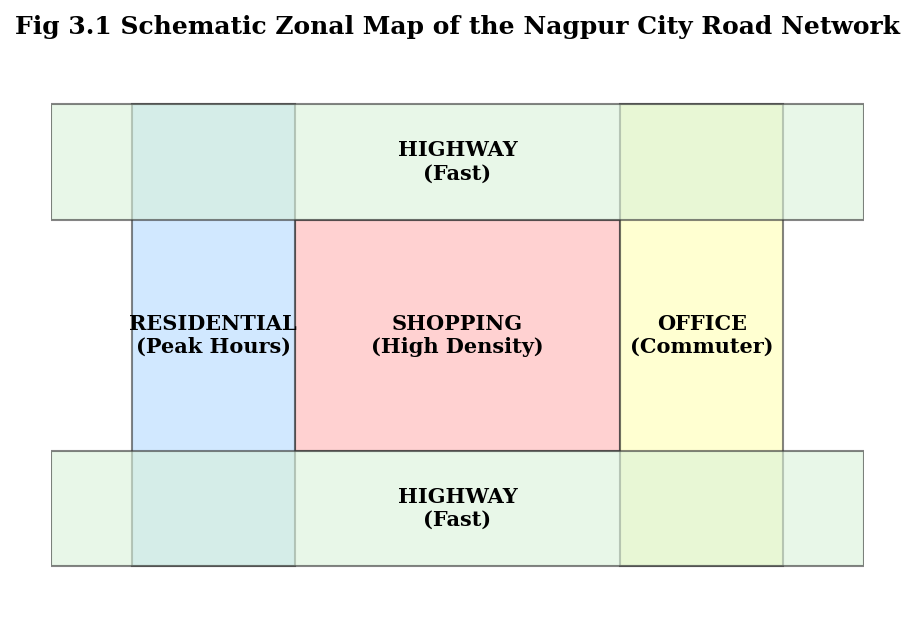
\includegraphics[width=0.85\textwidth]{images/fig3_1_nagpur_zone_map.png}
    \caption{Schematic Zonal Map of the Nagpur City Road Network used in the Simulation}
    \label{fig:zone_map}
\end{figure}

% ================================================================
\section{PPO Agent State Space: The 25-Dimensional Vector}

% ----------------------------------------------------------------
\subsection{State Vector Design}

The Central PPO Brain observes the environment through a 25-dimensional state
vector at each dispatch decision point. The vector is normalized to the range
$[0, 1]$ for continuous features and uses circular encoding for time-based
features to preserve the periodicity of daily and weekly cycles. Table~\ref{tab:ppo_state}
lists all 25 dimensions.

\begin{table}[h!]
\centering
\caption{PPO Central Brain: 25-Dimensional State Vector}
\label{tab:ppo_state}
\begin{tabular}{|c|l|l|}
\hline
\textbf{Index} & \textbf{Feature Name}             & \textbf{Encoding} \\
\hline
1  & Truck fuel level                  & Normalized [0, 1]              \\
2  & Cargo RSL                         & Normalized [0, 1]              \\
3  & Distance to destination           & Normalized [0, 1]              \\
4  & Current traffic density           & Normalized [0, 1]              \\
5  & Weather severity                  & Normalized [0, 1]              \\
6  & Sin(hour of day)                  & Circular encoding [-1, 1]      \\
7  & Cos(hour of day)                  & Circular encoding [-1, 1]      \\
8  & Sin(day of week)                  & Circular encoding [-1, 1]      \\
9  & Cos(day of week)                  & Circular encoding [-1, 1]      \\
10 & Number of active road accidents   & Normalized count [0, 1]        \\
11 & Fleet average fuel level          & Normalized [0, 1]              \\
12 & Fleet average RSL                 & Normalized [0, 1]              \\
13 & Pending orders in queue           & Normalized [0, 1]              \\
14 & Warehouse stock level             & Normalized [0, 1]              \\
15 & Road type of current edge         & One-hot (3 classes)            \\
16 & Zone of current edge              & One-hot (4 classes)            \\
17 & Estimated ETA to destination      & Normalized [0, 1]              \\
18 & Last reward received              & Normalized                     \\
19 & Number of trucks currently idle   & Normalized [0, 1]              \\
20 & Trucks currently in transit       & Normalized [0, 1]              \\
21--25 & Fleet utilization metrics     & Normalized [0, 1]              \\
\hline
\end{tabular}
\end{table}

% ================================================================
\section{ETA Forecaster Feature Engineering: The 8-Dimensional Vector}

% ----------------------------------------------------------------
\subsection{Feature Vector Design}

The ETA Forecaster predicts the travel time of a truck along a specific road
segment based on current conditions. The feature vector was upgraded from a
5-dimensional baseline (which only included time, weather, density, and road type)
to an 8-dimensional vector that incorporates circular day-of-week encoding and
geographic zone information. Table~\ref{tab:eta_features} lists all 8 dimensions
and the rationale for each.

\begin{table}[h!]
\centering
\caption{ETA Forecaster: 8-Dimensional Feature Vector}
\label{tab:eta_features}
\begin{tabular}{|c|l|p{7cm}|}
\hline
\textbf{Index} & \textbf{Feature}         & \textbf{Rationale} \\
\hline
1 & Sin(time of day)          & Captures morning rush hour cyclicality without discontinuity at midnight \\
\hline
2 & Cos(time of day)          & Paired with sin for complete circular time encoding \\
\hline
3 & Sin(day of week)          & Captures weekday-versus-weekend traffic differences \\
\hline
4 & Cos(day of week)          & Paired with sin for complete weekly cycle encoding \\
\hline
5 & Weather severity          & Rain, fog, and extreme heat directly increase travel time \\
\hline
6 & Traffic density           & Primary linear predictor of segment travel time \\
\hline
7 & Road type                 & Highway segments are faster than residential streets at all times \\
\hline
8 & Geographic zone           & Different zones have distinct peak-hour traffic profiles \\
\hline
\end{tabular}
\end{table}

The circular encoding of time (features 1--4) is necessary because of the
periodic nature of daily and weekly cycles. A na{\"i}ve encoding that represents
Monday as 1 and Sunday as 7 would imply that Monday is ``close'' to Tuesday but
``far'' from Sunday, when in reality Monday and Sunday are adjacent days in the
weekly cycle. The sin/cos encoding resolves this by mapping each day to a point on
a unit circle, where adjacent days remain close in the encoded space regardless
of their numerical labels.

% ----------------------------------------------------------------
\subsection{Online Learning and Dimension Compatibility}

The ETA Forecaster trains incrementally using \texttt{partial\_fit()}, updating
after every road segment traversal during the simulation. To ensure compatibility
across simulation runs, a dimension check is performed at startup: if a saved
model checkpoint was trained on the old 5-dimensional feature vector, it is
discarded and the model is reset to the new 8-dimensional configuration. This
prevents silent inference errors from feature mismatches.

% ================================================================
\section{Reward Function Design and Normalization}

% ----------------------------------------------------------------
\subsection{Components of the Reward Function}

The PPO agent receives a scalar reward at each dispatch decision step. The reward
is composed of four components:

\begin{equation}
    R = w_d \cdot \mathbb{1}[\text{delivery}] - w_f \cdot \Delta\text{fuel} - w_r \cdot \Delta\text{RSL} - w_s \cdot \mathbb{1}[\text{stockout}]
\end{equation}

where $w_d$ is the delivery completion bonus weight, $w_f$ is the fuel penalty
weight, $w_r$ is the cargo decay penalty weight, and $w_s$ is the stockout penalty
weight. $\Delta\text{fuel}$ and $\Delta\text{RSL}$ are the changes in fuel level
and cargo RSL during the dispatch episode.

% ----------------------------------------------------------------
\subsection{The 5:1 Normalization Problem and Solution}

Without careful calibration of the penalty weights, the PPO agent consistently
converged to a fuel-conservative policy and ignored RSL penalties. An analysis of
the physical magnitudes of these two quantities revealed the root cause. In a
typical delivery trip across Nagpur, a truck consumes approximately 10--15\% of
its fuel capacity, while the cargo RSL declines by only 1--2\% over the same
period (given a 7-day initial shelf life and a 1--2 hour transit time). If both
penalties are given equal weights, the fuel penalty dominates the reward signal by
a factor of approximately 10:1, causing the optimizer to focus entirely on fuel
conservation.

To correct this imbalance, the freshness penalty weight $w_r$ was set to 50.0
and the fuel penalty weight $w_f$ was set to 10.0, establishing a 5:1 ratio. This
equalizes the expected contribution of each penalty to the total reward signal per
trip, allowing the PPO agent to treat fuel efficiency and cargo freshness as equally
important objectives. The result is a policy that dynamically selects the
appropriate mode (Fuel-Priority, RSL-Priority, or Speed-Priority) based on the
current state of each truck, rather than defaulting to a single fixed strategy.

% ================================================================
\vspace{1cm}
\noindent \textbf{Chapter Summary:} This chapter described the two types of
telemetry data produced by the simulation engine, the Nagpur city road network
model with its four zone classifications, and the state representation used by
each AI component. The 25-dimensional PPO state vector captures the full context
needed for macro-level strategy decisions, while the 8-dimensional ETA feature
vector enables spatial-temporal travel time prediction. The reward normalization
framework establishes the 5:1 weighting ratio required for the PPO agent to learn
balanced, multi-objective routing policies. The next chapter describes the full
design and implementation of each system component.
